\documentclass[aps,prx,reprint,superscriptaddress,longbibliography,floatfix]{revtex4-2}

\usepackage[T1]{fontenc}
\usepackage[utf8]{inputenc}
\usepackage{amsmath,amssymb,bm,graphicx,physics,xcolor,hyperref}
\graphicspath{{figures/main/}{figures/supplementary/}}

\begin{document}

\title{Finite Dynamical Resource Manifolds from Non-Adiabatic Curvature and Operator Topology}

\author{Hang Hu}
\affiliation{Digital Technologies, National Research Council of Canada, 222 College Street, Toronto, ON M5T 3J1, Canada}
\author{Hsu Kiang Ooi}
\affiliation{Digital Technologies, National Research Council of Canada, 222 College Street, Toronto, ON M5T 3J1, Canada}
\author{Anguang Hu}
\affiliation{Suffield Research Centre, Defence Research and Development Canada, PO Box 4000 Station Main, Medicine Hat, Alberta T1A 8K6, Canada}

\begin{abstract}
Quantum resources such as entanglement, coherence, superposition, and interference are often discussed in terms of global enhancement, but in realistic systems their usefulness is usually confined to finite dynamical regimes in which competing mechanisms remain jointly effective. Here we formulate Entanglement-Dynamic Topology (EDT) as a quantitative framework for identifying such finite resource manifolds. The microscopic diagnostic is non-adiabatic electron--phonon curvature, defined through second-order variations of electronic energies with respect to normal-mode coordinates, which organizes correlated dynamics near degeneracies. As a main material example, we analyze K$_3$C$_{60}$ and identify a finite EDT window by fitting paired curvature branches to a local quadratic form with a residual threshold. To test the same finite-regime logic in a minimal dynamical setting, we study a four-qubit plaquette Hamiltonian in which loop-induced interactions produce an interior optimum of operator spreading and long-time correlation retention. We further examine robustness under Trotterized implementation and bounded circuit depth, showing that the optimal regime persists under approximate compilation. Finally, we use NV-center XY8 sensing as a control-oriented case study in which sweeps over pulse spacing and sequence depth reveal a finite optimum set by the balance among filter response, coherence, pulse fidelity, and readout overhead. Taken together, these results support a finite-regime view of quantum resource organization that links non-adiabatic curvature diagnostics, minimal dynamical models, and sensing-oriented control landscapes within a common quantitative framework.
\end{abstract}

\maketitle

\section{Introduction}

Quantum computation, sensing, and materials design fundamentally depend on the controlled use of quantum resources, including entanglement, coherence, superposition, and interference~\cite{NielsenChuang,Horodecki2009,Streltsov2017}. In most current approaches, these resources are treated as quantities to be maximized, leading naturally to strategies that explore increasingly large Hilbert spaces~\cite{Preskill2018,Arute2019}. While powerful in principle, this paradigm introduces severe scaling challenges and often obscures the physical structure underlying useful quantum dynamics~\cite{Eisert2010,Altman2015}.

An alternative perspective is that quantum advantage arises not from the size of Hilbert space, but from the \emph{organization} of quantum resources within it~\cite{Amico2008,Swingle2018}. In this view, the central problem is not to generate maximal entanglement, but to engineer entanglement that is structured, localized, and aligned with the geometry of the task~\cite{Verstraete2008,Orus2014}. This shift reframes quantum control as a problem of resource organization rather than resource amplification. Useful quantum dynamics are then those that remain confined to structured manifolds where entanglement, interference, and correlation are jointly optimized~\cite{KimHuse2013,Choi2016}.

Here we introduce Entanglement-Dynamic Topology (EDT) as a unifying framework for programmable quantum resource engineering, building on recent developments in curvature-driven and topologically structured quantum dynamics~\cite{Hu2024_ACP,Hu2025_APQ,Hu2026_JPCM}. EDT describes a regime of quantum dynamics in which resources are simultaneously \emph{structured, interacting, topological, and dynamical}. Structure, arising from symmetry, constrains quantum states into reduced manifolds~\cite{Wigner1959,Georgi1999}. Interaction, driven by non-adiabatic coupling such as electron--phonon interaction, generates and redistributes entanglement~\cite{Mead1979,Yarkony1996}. Topology organizes this structure through nodes, poles, and vortex-like configurations in parameter space~\cite{Berry1984,Xiao2010}. Dynamics, through modulation of band energies and electronic potentials, renders these manifolds controllable and programmable~\cite{Bukov2015,Eckardt2017}.

A key feature of EDT is that it defines a finite regime rather than a fine-tuned point. Within this regime, quantum dynamics exhibit coherent, structured behavior, while outside it the dynamics become either weakly correlated or overdriven and incoherent~\cite{Larkin1969,Swingle2018}. This regime-based perspective provides a robust and experimentally meaningful foundation for quantum resource engineering, in contrast to approaches that rely on asymptotic scaling or finely tuned optimality.

To connect this framework to real physical systems, we first develop a data-driven method for identifying EDT directly from electronic-structure observables. Using K$_3$C$_{60}$ as the main material example, we analyze curvature-resolved band structure and show that EDT emerges as a finite momentum interval in which paired curvature branches admit a consistent local quadratic description. Supplementary archived comparison datasets for V, Na, LaH$_{10}$, and YBa$_2$Cu$_3$O$_7$ are then used as portability checks of the same diagnostic rather than as co-equal material claims. This provides an operational criterion for detecting EDT and establishes a direct link between microscopic electronic structure and structured quantum resources~\cite{Gunnarsson1997,Capone2009}.

We then show that this regime arises generically in a minimal dynamical model, where loop-induced operator spreading remains structured and compatible with persistent many-body correlation, and that it remains robust under parameter variation, bounded circuit complexity, and approximate implementation~\cite{Lloyd1996,Childs2019}. Finally, we demonstrate the same finite-regime logic in NV-center XY8 sensing, where optimal performance emerges from balancing filter response, coherence, pulse fidelity, and readout overhead within a bounded control window~\cite{Degen2017,Barry2020,Casola2018}.

\section{Finite-regime definition of entanglement-dynamic topology}

We define Entanglement-Dynamic Topology (EDT) as a \emph{finite parameter window} in which a system supports simultaneously structured, compatible, and dynamically useful quantum-resource behavior. The relevant control coordinate is denoted generically by $x$, where $x$ may represent momentum $k$, a phonon normal-mode coordinate $Q$, loop or interaction strength $\lambda$, circuit depth, pulse number $N$, pulse spacing $\tau$, or another experimentally accessible control variable. In this sense, EDT is not tied to a single platform-specific parameterization; it is a regime criterion applied to whichever coordinate organizes the competition between structure generation and resource degradation.

The EDT regime is defined as the set
\begin{equation}
\Delta_{\rm EDT}
=
\{x: S_{\rm pair}(x) > S_{\rm pair}^{(0)},
R_{\rm quad}(x) < R_{\rm quad}^{(0)},
S_{\rm dyn}(x) > S_{\rm dyn}^{(0)} \},
\end{equation}
where each inequality expresses a measurable or computable condition for finite-regime viability.

The first term, $S_{\rm pair}(x)$, is a curvature-pairing or branch-compatibility score. In materials examples, it quantifies how well paired curvature branches remain mutually compatible within a local description near a degeneracy or avoided crossing. In dynamical settings, it can be interpreted more generally as a compatibility measure between the relevant structured branches or channels supporting the candidate regime. The reference value $S_{\rm pair}^{(0)}$ sets the minimum compatibility required for the regime to be considered organized rather than accidental.

The second term, $R_{\rm quad}(x)$, is the residual error of a local quadratic model. It measures how well the relevant structure can be approximated by a stable local expansion around the candidate operating point. In the K$_3$C$_{60}$ analysis, this is the residual associated with paired quadratic fits to curvature branches. The threshold $R_{\rm quad}^{(0)}$ therefore separates regions where the local model remains coherent from regions where the structure becomes too irregular, too sharp, or too weakly organized to support a finite EDT window.

The third term, $S_{\rm dyn}(x)$, is a dynamical resource score. Its exact form depends on the platform. In the plaquette model, it is built from operator spreading and long-time correlation retention. In sensing problems, it may be a filtered response or sensitivity proxy combining signal accumulation with coherence and control fidelity. In all cases, $S_{\rm dyn}(x)$ is intended to capture whether the candidate region is not only geometrically structured but also dynamically useful. The threshold $S_{\rm dyn}^{(0)}$ enforces that the regime remain operationally relevant rather than merely geometrically identifiable.

When robustness information is available, we also introduce an optional score $S_{\rm robust}(x)$ measuring stability under threshold changes, parameter perturbations, or approximate implementation such as Trotterization. This quantity is not required to identify an EDT window at the most basic level, but it is useful for ranking candidate regimes by their resilience to modeling choices and control imperfections.

To summarize these ingredients in a single bounded diagnostic, we define a composite normalized score
\begin{equation}
S_{\rm EDT}(x) = S_{\rm pair}(x)\,S_{\rm quad}(x)\,S_{\rm dyn}(x)\,S_{\rm robust}(x),
\end{equation}
with
\begin{equation}
S_{\rm quad}(x) = \exp[-R_{\rm quad}(x)/R_0],
\end{equation}
where $R_0$ sets the residual scale. This choice ensures that improved local quadratic consistency increases the score monotonically while large residuals suppress it smoothly rather than through a discontinuous rule. When an explicit robustness measure is not available, one may set $S_{\rm robust}(x)=1$ and retain the three-factor finite-regime diagnostic.

Within this formulation, EDT is identified not by the maximization of any single quantity, but by the existence of an \emph{interior region} in control space where branch compatibility remains high, local structure remains well described, and dynamical usefulness remains above threshold. The resulting window is finite by construction: outside it, at least one of the conditions defining $\Delta_{\rm EDT}$ fails.

\paragraph*{Clarification.}

EDT is not a new microscopic interaction and not a new quantum resource type. It is a finite-regime organization principle identifying where existing quantum resources are simultaneously generated, structured, and dynamically stable.

\subsection{Physical Origin and Organization}

Within the present manuscript, the microscopic origin of the finite-regime structure is non-adiabatic coupling between electronic and lattice degrees of freedom~\cite{Mead1979,Yarkony1996,Giustino2017}. Near degeneracies and band crossings, the second-order response of electronic energies to normal-mode coordinates generates curvature fields that organize the local structure of the coupled manifold. These curvature fields provide the main materials-side diagnostic used below in K$_3$C$_{60}$, where the finite EDT window is extracted through paired curvature fits and residual thresholding.

The same finite-regime logic extends naturally beyond momentum-space diagnostics. In the plaquette model, the control coordinate is the loop strength $\lambda$, and the relevant dynamical score is built from operator spreading and long-time correlation persistence. In the NV XY8 case study, the control coordinates are pulse number $N$ and pulse spacing $\tau$, and the dynamical score is replaced by a sensing-oriented resource proxy combining filter response, coherence, pulse fidelity, and duty-cycle overhead. These examples differ in physical realization, but they share the same finite-window definition.

\begin{figure*}[t]
\centering
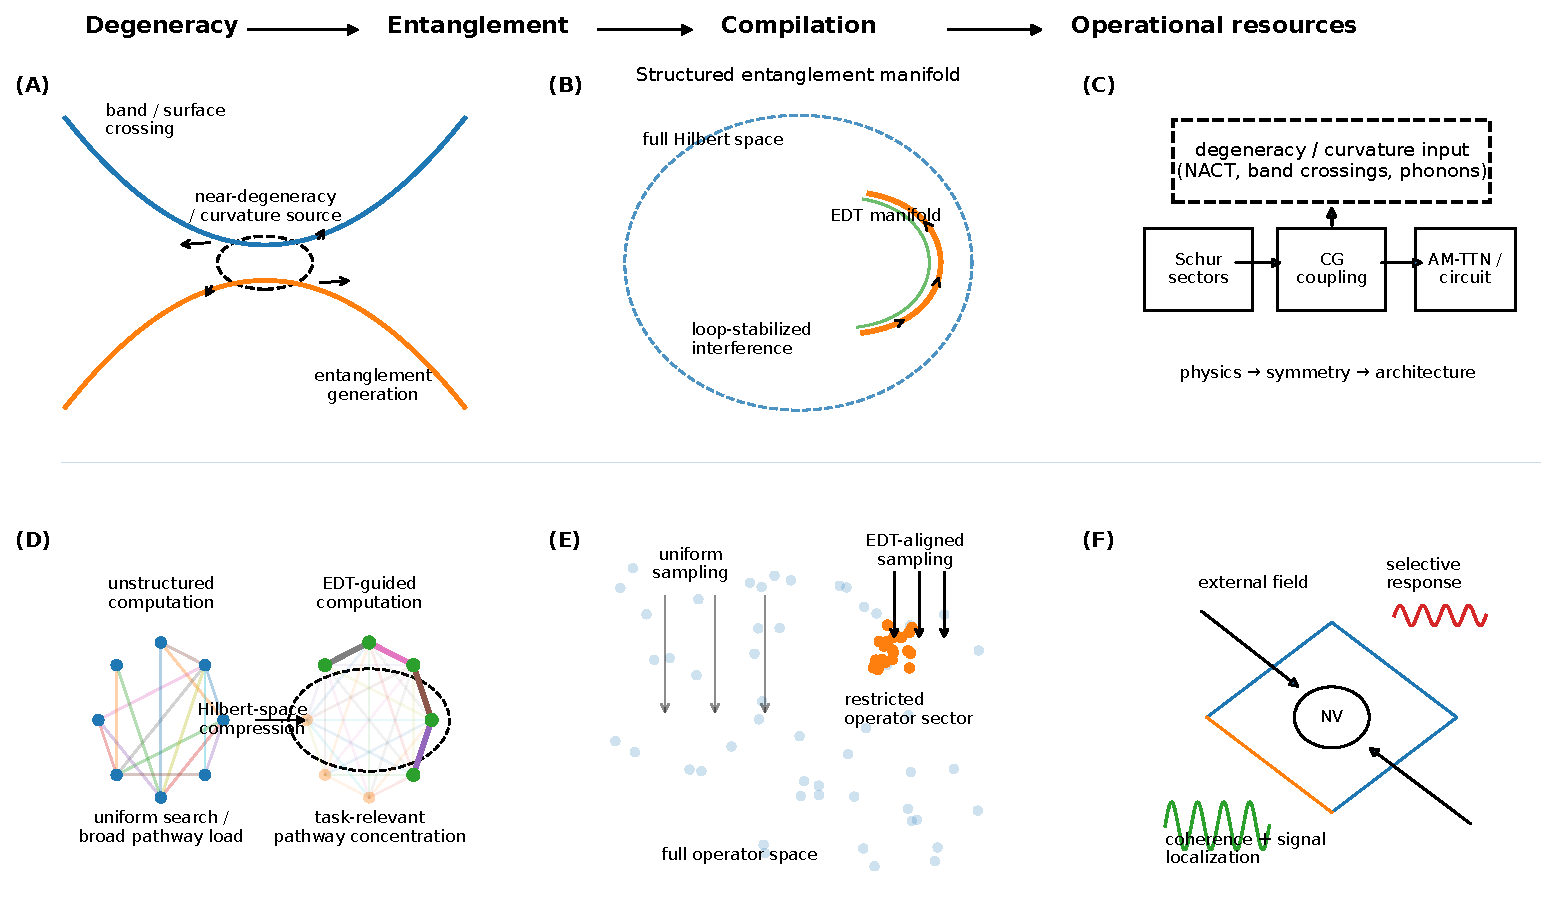
\includegraphics[width=0.95\linewidth]{fig1_edt_framework_camera_ready.pdf}
\caption{\textbf{Physical origin and organization of EDT.}
(A) Near degeneracies and band crossings act as curvature sources, where non-adiabatic coupling generates entanglement.
(B) A structured entanglement manifold is embedded within the full Hilbert space and stabilized by loop-induced interference.
(C) Physical structure can be compiled into symmetry-adapted architectures, including Schur sectors, Clebsch-Gordan coupling, and circuit representations.
(D) EDT-guided evolution concentrates dynamics into structured pathways rather than unstructured Hilbert-space exploration.
(E) Task-relevant operator sectors can be selectively sampled under EDT alignment.
(F) In sensing platforms, structured manifolds enable selective response and coherence localization.}
\label{fig:edt_concept}
\end{figure*}

\paragraph*{From non-adiabatic coupling to an effective EDT Hamiltonian.}

Starting from the electron--phonon Hamiltonian
\begin{equation}
H = H_e(\mathbf{r};\{Q_\alpha\}) + \sum_\alpha \left(\frac{P_\alpha^2}{2M_\alpha} + \frac{1}{2} M_\alpha \omega_\alpha^2 Q_\alpha^2\right),
\end{equation}
non-adiabatic effects arise from the dependence of the electronic Hamiltonian on normal-mode coordinates $Q_\alpha$~\cite{BornOppenheimer1927,Mead1979,Yarkony1996}. Expanding $H_e$ to second order,
\begin{equation}
H_e(\{Q_\alpha\}) \approx H_e^{(0)} + \sum_\alpha Q_\alpha \,\partial_\alpha H_e + \frac{1}{2}\sum_{\alpha\beta} Q_\alpha Q_\beta \,\partial_\alpha \partial_\beta H_e,
\end{equation}
and projecting onto an adiabatic electronic basis $\{|n\rangle\}$ yields NACT matrix elements
\begin{equation}
A^{(\alpha)}_{mn} = \langle m | \partial_{Q_\alpha} | n \rangle,
\end{equation}
which generate off-diagonal mixing and geometric phases~\cite{Berry1984}. Eliminating fast phonon coordinates produces an effective electronic Hamiltonian with curvature-mediated interactions~\cite{SchriefferWolff1966,LangFirsov1962},
\begin{equation}
H_{\mathrm{eff}} \simeq H_0 + \sum_{\langle i,j\rangle} J_{ij}\, Z_i Z_j + \sum_p \lambda_p\, W_p,
\end{equation}
where $J_{ij}$ arises from second-order curvature processes and $W_p$ denotes loop operators generated by multi-mode interference of NACT fields.

At the operational level, these structures define a computational framework. The structured manifold can be compiled into symmetry-adapted architectures, including Schur-sector decompositions, Clebsch--Gordan coupling trees, and tensor-network representations, enabling Hilbert-space compression and concentration of dynamics along task-relevant pathways~\cite{Bacon2006}. In this way, the finite-regime definition of EDT connects microscopic curvature diagnostics to dynamical models and platform-level control studies within a single quantitative language.

\section{Curvature diagnostic for non-adiabatic resource manifolds}

The microscopic diagnostic used in the present work is the electronic curvature of band $n$ with respect to phonon normal-mode coordinate $Q_\alpha$,
\begin{equation}
\kappa_{n\alpha}(k)=\frac{\partial^2 E_n(k,Q_\alpha)}{\partial Q_\alpha^2}.
\end{equation}
This quantity measures the second-order response of the electronic structure to lattice displacement and provides a direct non-adiabatic diagnostic near degeneracies and avoided crossings~\cite{Mead1979,Yarkony1996,Giustino2017}. In practice, $\kappa_{n\alpha}(k)$ is computed numerically from displaced calculations using either centered finite differences or local fits to displaced energy data. For a symmetric three-point stencil at displacements $(-\Delta Q,0,+\Delta Q)$, one may write
\begin{equation}
\kappa_{n\alpha}(k)\approx
\frac{E_n(k,-\Delta Q)-2E_n(k,0)+E_n(k,+\Delta Q)}{(\Delta Q)^2},
\end{equation}
while higher-order fitted-displacement schemes can be used when additional displaced configurations are available.

Near a candidate EDT region, we analyze paired curvature branches using the form
\begin{equation}
\kappa_\pm(k)
=
\kappa_0
\pm a(k-k_0)^2
+
\epsilon_\pm(k),
\end{equation}
where $\kappa_0$ is the common offset, $a$ sets the local quadratic scale, $k_0$ is the center of the paired structure, and $\epsilon_\pm(k)$ are residual deviations from the shared quadratic model. The corresponding normalized residual is defined as
\begin{equation}
R_{\rm quad}
=
\frac{
\sqrt{\sum_k |\epsilon_+(k)|^2 + |\epsilon_-(k)|^2}
}{
\sqrt{\sum_k |\kappa_+(k)|^2 + |\kappa_-(k)|^2}
}.
\end{equation}
This quantity provides a scale-independent measure of how well the paired branches admit a coherent local quadratic description.

The EDT momentum window is then defined as
\begin{equation}
\Delta k_{\rm EDT}
=
\max_{\Delta k}
\left\{
\Delta k:
R_{\rm quad}(\Delta k)<R_{\rm th}
\right\},
\end{equation}
where $R_{\rm th}$ is a prescribed residual threshold. In words, $\Delta k_{\rm EDT}$ is the largest momentum interval over which the paired curvature branches remain compatible with the local quadratic model. This provides a falsifiable and reproducible criterion for identifying finite non-adiabatic resource manifolds in band-structure data.

To make this diagnostic directly reproducible in the code base, we provide a dedicated module, \texttt{edt.curvature}; the implementation is in \texttt{src/edt/curvature.py}. The module includes utilities to load tabulated band data, compute curvature from displaced calculations, fit paired quadratic branches, evaluate the normalized residual, extract the EDT window from a thresholded residual profile, and estimate uncertainty in the extracted window through bootstrap resampling.

\section{Curvature-defined EDT window in K$_3$C$_{60}$}

K$_3$C$_{60}$ is a useful materials test case for the present diagnostic because it combines narrow near-Fermi bands with strong electron--phonon coupling in a molecular solid, so finite non-adiabatic structure is expected without having to invoke a broad many-parameter model~\cite{Gunnarsson1997,Capone2009}. In the present manuscript, K$_3$C$_{60}$ is the main material example used to anchor EDT to a falsifiable microscopic quantity rather than to a qualitative narrative. The role of Fig.~\ref{fig:k3c60_edt_window} is therefore specific: it shows exactly which curvature pair is analyzed, how the local quadratic window is extracted, and how sensitive the extracted window is to analysis choices. The Supplement places this main example in a broader archived-controls context using representative comparison datasets from V, Na, LaH$_{10}$, and YBa$_2$Cu$_3$O$_7$.

The reproducible bundle for this case study contains two complementary data products. Panel (a) uses the archived near-Fermi band-structure figure \texttt{figures/supplementary/K3C60-bands.pdf} as band-context reference for the same calculation. Panels (b)--(e) are generated directly from the bundled curvature export \texttt{data/k3c60/tmp.agr} by running \texttt{python scripts/make\_fig2\_k3c60\_edt.py}. The metadata embedded in the AGR file identify the observable as a mode-resolved curvature trace, $\partial^2 E_n(k)/\partial q^2$, evaluated along the $\Gamma$--X--L--W--$\Gamma$ path. The archived companion figure and caption identify the representative normal mode as \texttt{m120} at $1090.35~\mathrm{cm}^{-1}$.

Curvature is extracted from displaced electronic-structure calculations as the second derivative of the band energy with respect to phonon normal-mode coordinate, as defined in the preceding curvature-diagnostic section; the bundled archive provides the resulting mode-resolved curvature traces rather than the full family of displaced calculations. Within that exported dataset, we analyze Bands 208 and 209 in the archived numbering because they form the clearest opposite-sign branch pair in the selected momentum interval. Operationally, the pair is identified by locating a local minimum in one branch and a local maximum in the other at the same momentum point inside the analysis window. For the nominal window used in Fig.~\ref{fig:k3c60_edt_window}, both extrema occur near $k \approx 0.818$, and the corresponding local quadratic fits give a shared center $k_0 = 0.823$.

The finite EDT window is then defined from the paired-branch residual diagnostic. Using the analysis slice indexed by 150--281 in the archived trace, a nominal local fit half-window of 18 points, and a residual threshold $R_{\rm th}=0.08$, we obtain a finite window extending from $k_{\rm left}=0.742$ to $k_{\rm right}=0.896$, corresponding to $\Delta k_{\rm EDT}=0.154$. Panel (d) makes this definition explicit by plotting the branch-resolved residuals and shading the interval over which the two branches remain simultaneously compatible with the local quadratic description. This is the quantity we use as the curvature-defined EDT window in the K$_3$C$_{60}$ analysis.

The main robustness checks are summarized in panel (e) and in Supplementary Fig.~S5. Varying the residual threshold from 0.04 to 0.18 changes the extracted width only from 0.137 to 0.178, while varying the fit-window size from 10 to 28 points changes the width from 0.127 to 0.199. Subsampling the $k$ grid from 131 points down to 33 points gives widths between 0.144 and 0.164. A local-fit bootstrap around the selected pair gives a 95\% confidence interval of $[0.147,\,0.158]$ for the nominal width. We also compare neighboring band-pair choices, which shows that pair selection is a real analysis axis rather than a hidden fixed choice: the archived visible pair, Bands 208/209, gives the nominal window, while nearby pairs give different finite widths. The only robustness axis that cannot be reproduced from the bundled archive is a displacement-amplitude sweep, because the archived dataset contains one exported curvature product rather than a matched family of displaced calculations at multiple amplitudes. This is why the supplementary cross-material datasets are interpreted conservatively as diagnostic portability checks based on explicit representative candidate pairs, rather than as material-by-material reconstructions with identical evidentiary weight.

\begin{figure*}[t]
\centering
\begin{minipage}{0.48\linewidth}
\textbf{(a)}\\[-0.4em]
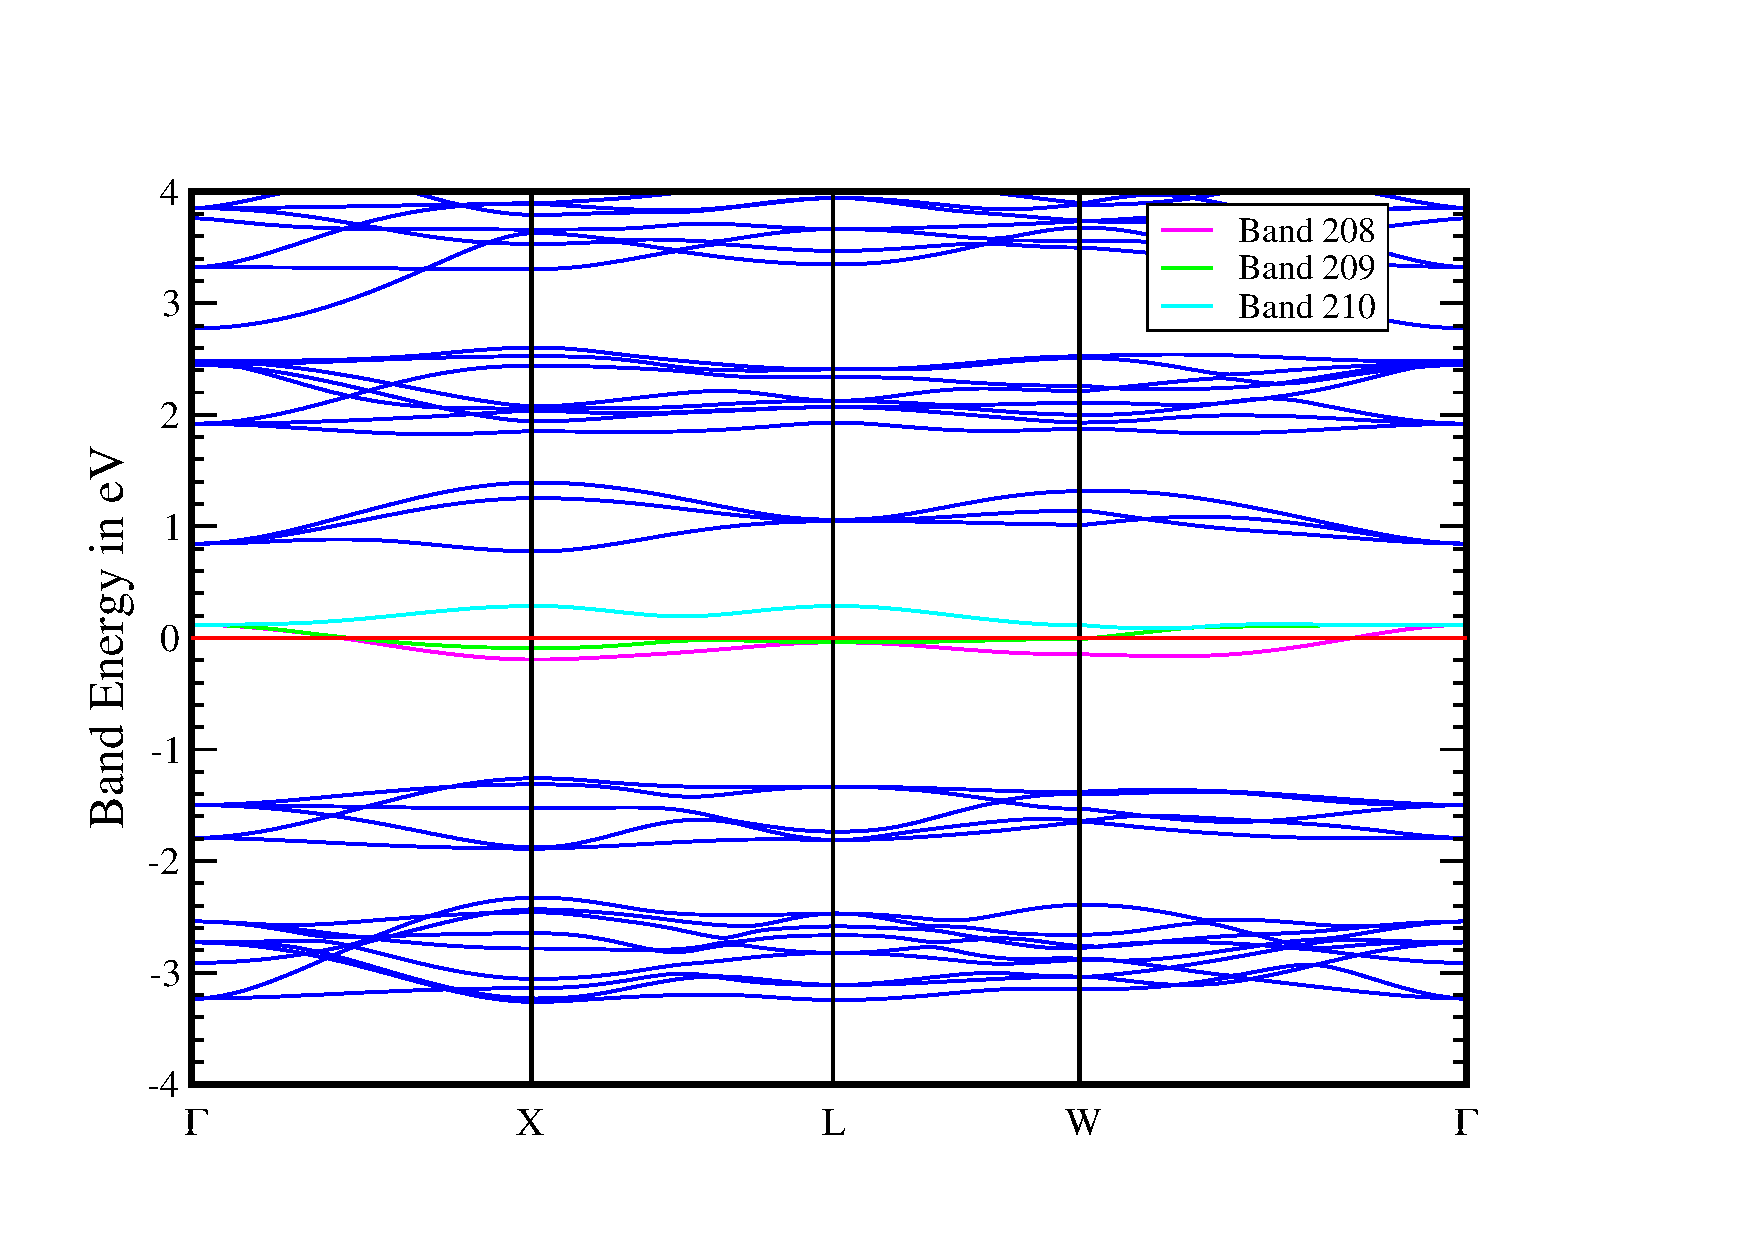
\includegraphics[width=\linewidth]{K3C60-bands.pdf}
\end{minipage}\hfill
\begin{minipage}{0.48\linewidth}
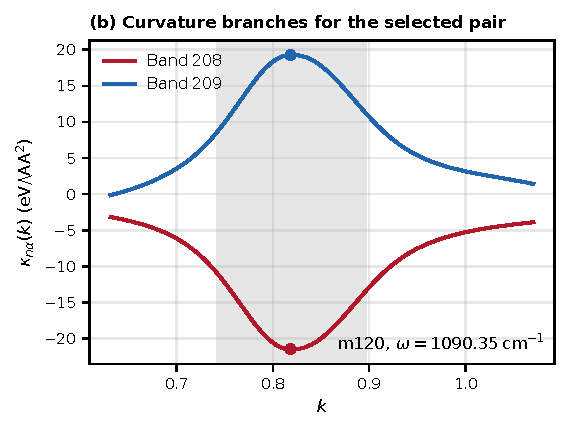
\includegraphics[width=\linewidth]{figure2_k3c60_panel_b_curvature.pdf}
\end{minipage}

\vspace{0.5em}

\begin{minipage}{0.48\linewidth}
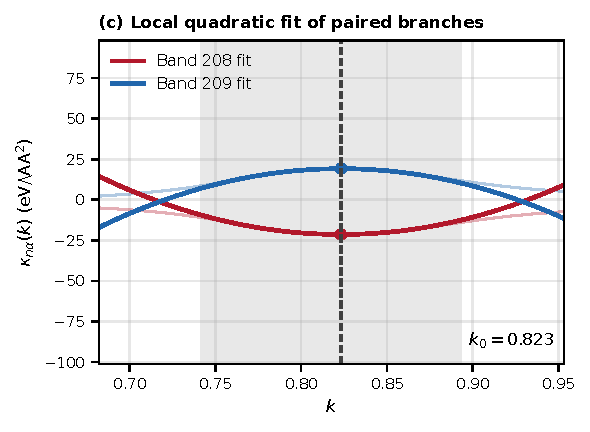
\includegraphics[width=\linewidth]{figure2_k3c60_panel_c_fit.pdf}
\end{minipage}\hfill
\begin{minipage}{0.48\linewidth}
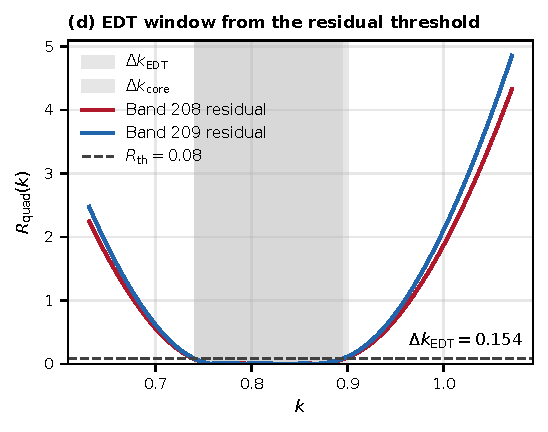
\includegraphics[width=\linewidth]{figure2_k3c60_panel_d_window.pdf}
\end{minipage}

\vspace{0.5em}

\begin{minipage}{0.48\linewidth}
\centering
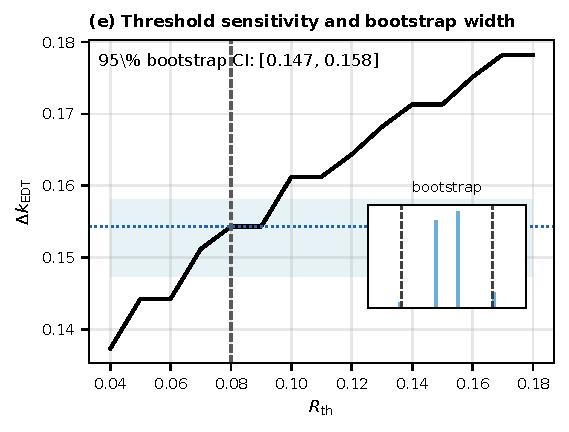
\includegraphics[width=\linewidth]{figure2_k3c60_panel_e_bootstrap.pdf}
\end{minipage}
\caption{\textbf{Curvature-defined EDT window in K$_3$C$_{60}$.}
(a) Near-Fermi band-structure context for cubic K$_3$C$_{60}$ from the archived companion band plot of the same calculation. (b) Mode-resolved curvature $\kappa_{n\alpha}(k)$ for the selected paired branches, Bands 208 and 209, for mode \texttt{m120} at $1090.35~\mathrm{cm}^{-1}$. (c) Local quadratic fits for the paired branches, yielding a shared center near $k_0=0.823$. (d) Branch-resolved normalized residuals and the nominal EDT window extracted at $R_{\rm th}=0.08$, giving $\Delta k_{\rm EDT}=0.154$. (e) Threshold sensitivity of the extracted width together with a local-fit bootstrap inset. Panels (b)--(e) are generated from \texttt{data/k3c60/tmp.agr} by \texttt{scripts/make\_fig2\_k3c60\_edt.py}.}
\label{fig:k3c60_edt_window}
\end{figure*}

\section{Minimal plaquette model of finite EDT dynamics}

The plaquette Hamiltonian is a minimal model designed to capture the same structural ingredients identified in the curvature analysis: local interactions, loop-induced nonlocal correlations, and finite-regime operator spreading. It is not claimed to be a quantitatively fitted Hamiltonian for K$_3$C$_{60}$ unless explicit parameter fitting is provided. In this sense, the plaquette model plays the role of a controlled dynamical analog of the curvature-defined finite window rather than a microscopic materials model.

The minimal Hamiltonian is
\begin{equation}
H =
J \sum_{\langle i,j\rangle} Z_i Z_j
+
h \sum_i X_i
+
\lambda Z_0 Z_1 Z_2 Z_3.
\end{equation}
The first term provides local nearest-neighbor Ising interactions on the four-site plaquette, the transverse-field term drives operator growth away from a static computational basis, and the four-body loop term generates the nonlocal interference structure that makes the finite EDT regime nontrivial. In the code base, this Hamiltonian is implemented directly in the minimal package \texttt{plaquette\_model}, which exposes exact evolution, OTOC evaluation, entanglement diagnostics, correlation tracking, and first-order Trotter evolution as separate reproducible functions.

The purpose of this model is diagnostic rather than materials-specific. By sweeping the loop strength $\lambda$ and following the resulting time evolution, one can ask whether the same finite-regime logic seen in the K$_3$C$_{60}$ curvature window reappears dynamically: weak loop strength leaves correlations too local, strong loop strength overdrives the system into rapidly scrambled behavior, and an intermediate regime supports simultaneous operator spreading, persistent correlations, and moderate entanglement growth. That intermediate regime is the minimal dynamical analog of the finite EDT window.

In practice, the dynamical observables used below are the out-of-time-ordered correlator, nearest-neighbor two-point correlations, and subsystem entanglement entropy. These are combined into a composite dynamical score that is intentionally finite-regime in character: it rewards operator spreading and correlation retention while penalizing both trivial product-state dynamics and fully saturated scrambling. Exact time evolution and Trotterized evolution are both computed so that the finite EDT regime can be tested not only as a property of the Hamiltonian, but also as a feature that survives approximate implementation.

\section{Operator spreading and finite optimality}

The minimal plaquette model is used to test whether the finite-regime logic identified in the curvature analysis reappears in real-time dynamics. We therefore compute the dynamics as a function of the loop coupling $\lambda$ and ask whether operator spreading, correlation persistence, and entanglement organization all remain simultaneously effective in a bounded interval rather than at the strongest available loop term.

Operator spreading is tracked through the out-of-time-ordered echo
\begin{equation}
F(t)
=
\langle W^\dagger(t)V^\dagger W(t)V\rangle,
\end{equation}
with the plotted OTOC metric defined as $1-\mathrm{Re}\,F(t)$. In the numerical sweep we average over three probe configurations: two computational-basis initial states and one $|+\!+\!+\!+\rangle$ state, together with distinct Pauli choices for $(W,V)$. This keeps the finite-optimality claim from depending on a single probe. Long-time correlation persistence is quantified by the late-time average of nearest-neighbor $ZZ$ correlators, while stability is quantified through a one-qubit entanglement factor that is largest at intermediate entropy and suppressed near both product-state and over-scrambled limits.

The resulting dynamical score is
\begin{equation}
S_{\rm dyn}(\lambda)
=
A_{\rm spread}(\lambda)\,
A_{\rm corr}(\lambda)\,
A_{\rm stability}(\lambda).
\end{equation}
Here $A_{\rm spread}$ is the normalized mid-time OTOC amplitude, $A_{\rm corr}$ is the normalized late-time correlation persistence, and $A_{\rm stability}$ is the intermediate-entropy factor extracted from the subsystem entanglement. This definition is intentionally finite-regime in character: it rewards spreading only when it coexists with correlation retention and dynamical stability.

Figure~\ref{fig:fig4_plaquette_dynamics} shows the three regimes clearly. For small $\lambda$, operator spreading remains weak and the OTOC grows only modestly. For an intermediate loop strength $\lambda^\star$, the OTOC develops strongly while long-time correlations remain appreciable and the entanglement remains in the structured intermediate range. For large $\lambda$, operator spreading is still present, but correlation persistence degrades and the combined score drops, indicating overdriven or scrambled dynamics rather than a useful finite EDT regime. For the nominal sweep shown in Fig.~\ref{fig:fig4_plaquette_dynamics}, with $J=0.4$ and $h=0.4$, the maximum occurs at $\lambda^\star = 0.8$, while representative small- and large-coupling points are $\lambda = 0.15$ and $\lambda = 1.25$, respectively.

The finite optimum is not a single-point artifact of the nominal controls. Panel (e) of Fig.~\ref{fig:fig4_plaquette_dynamics} shows the extracted $\lambda^\star$ under variation of the transverse field $h$ for several $J$ values. The optimum shifts with control parameters, as expected for a real dynamical landscape, but it remains interior over a substantial part of the sweep rather than collapsing to $\lambda=0$ or to the largest tested loop strength. This is the key dynamical result of the minimal model: finite EDT behavior appears as a bounded optimum in operator spreading and correlation persistence, not as monotonic improvement with increasing nonlocal control.

\begin{figure*}[t]
\centering
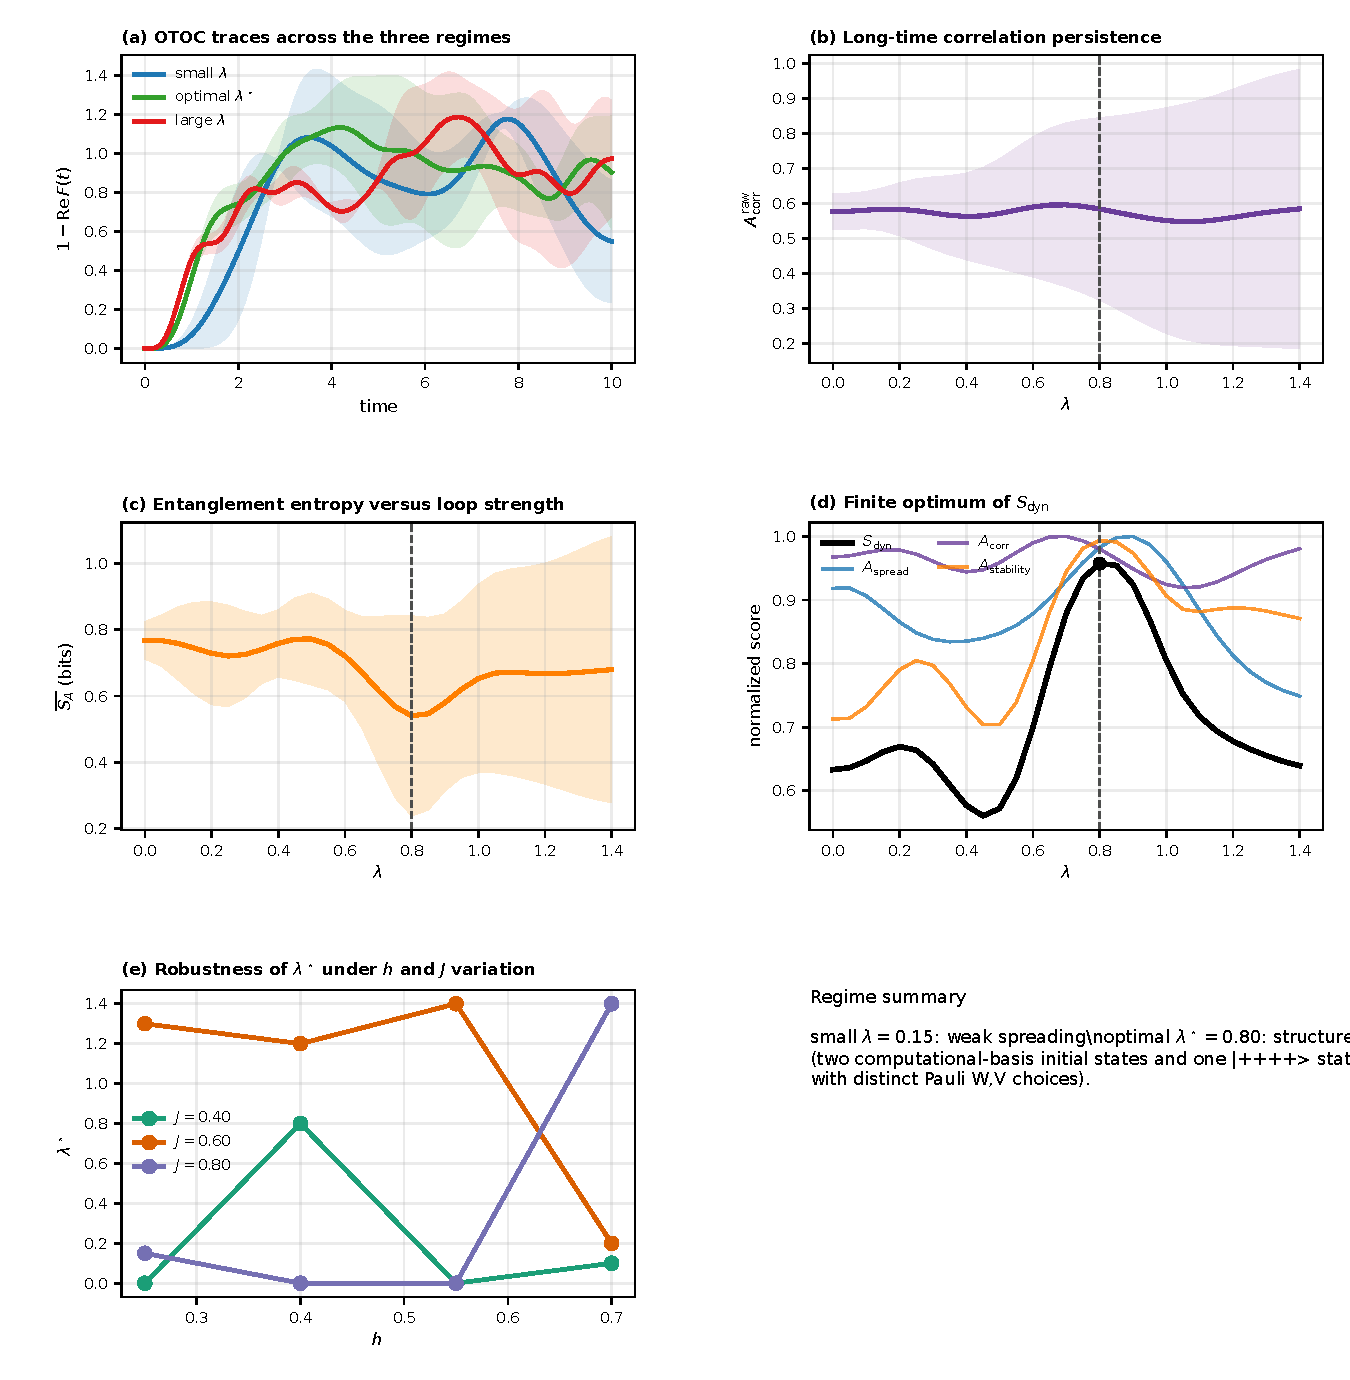
\includegraphics[width=0.96\linewidth]{fig4_plaquette_dynamics.pdf}
\caption{\textbf{Operator spreading and finite optimality in the minimal plaquette model.}
(a) Probe-averaged OTOC traces, plotted as $1-\mathrm{Re}\,F(t)$, for representative small, optimal, and large loop couplings. (b) Late-time nearest-neighbor correlation persistence versus $\lambda$. (c) One-qubit entanglement entropy versus $\lambda$. (d) Composite dynamical score $S_{\rm dyn}=A_{\rm spread}A_{\rm corr}A_{\rm stability}$, showing a finite optimum at intermediate loop strength. (e) Robustness of the optimal loop coupling $\lambda^\star$ under variation of $h$ for several fixed $J$ values. The figure is generated by \texttt{scripts/fig4\_plaquette\_dynamics.py}, and the processed sweep data are written to \texttt{data/processed/plaquette\_lambda\_sweep.csv}.}
\label{fig:fig4_plaquette_dynamics}
\end{figure*}

\section{NV XY8 Case Study}

The NV-center platform is used here as a control-oriented case study of EDT-style finite-regime optimization rather than as a direct experimental realization of the materials-side curvature diagnostic~\cite{Degen2017,Barry2020}. In NV--XY8 sensing protocols, performance is governed by a structured combination of resource factors, including filter gain $G(f)$, coherence time, pulse fidelity, and readout contrast. As shown in Fig.~\ref{fig:fig5_nvdemo}, these quantities do not improve monotonically with control parameters such as pulse number $N$ or spacing $\tau$. Instead, an optimal operating point emerges as a finite regime in which signal amplification, coherence preservation, and control accuracy are balanced~\cite{Casola2018}.

This behavior is directly analogous to the EDT regime identified in the plaquette-model analysis. Increasing control strength enhances sensitivity through improved filter response, but also accelerates decoherence and accumulates control errors. As a result, sensing performance exhibits a maximum within a finite window rather than at extreme parameter values. Within this regime, the sensor dynamics remain aligned with a structured manifold in control space, enabling both selective response and coherence localization~\cite{Degen2017,Barry2020}.

\subsection{Rate-Based Model}

Quantum sensing in NV-center ensembles is analyzed within a quantum resource engineering framework using a rate-based model (\texttt{nvratemodel} API) that maps experimental control parameters to effective quantum resources and sensing performance~\cite{NVRateModel2023,Degen2017,Barry2020}. For XY8 dynamical-decoupling sequences, the control parameter set is defined as
\begin{equation}
\mathcal{C} = \{P_{\mathrm{laser}},\, t_{\mathrm{read}},\, \Omega_{\mathrm{MW}},\, \tau,\, N_{\pi},\, B_0,\, T,\, \mathrm{strain}\},
\end{equation}
which determines initialization, control, and environmental conditions of the sensor~\cite{Casola2018}.

These controls are mapped onto an effective resource vector
\begin{equation}
\mathcal{R} = \{R_{\mathrm{ph}},\, C,\, T_2(N_{\pi}),\, \chi(\omega),\, \mathrm{duty}\},
\end{equation}
where $R_{\mathrm{ph}}$ is the detected photon rate, $C$ is the fluorescence contrast, $T_2(N_{\pi})$ is the coherence time under dynamical decoupling, $\chi(\omega)$ is the filter-function response, and $\mathrm{duty}$ accounts for initialization and readout overhead. The filter function is peaked near $\omega \simeq \pi/\tau$, enabling frequency-selective amplification of ac fields~\cite{Cywinski2008}.

Sensing performance is quantified by a sensitivity proxy $\eta_{\mathrm{AC}}(\omega)$, which scales approximately as
\begin{equation}
\eta_{\mathrm{AC}}(\omega) \propto \frac{1}{\chi(\omega)\,C\,\sqrt{R_{\mathrm{ph}}\,T_2(N_{\pi})}} \times f_{\mathrm{duty}},
\end{equation}
consistent with standard analyses of NV magnetometry sensitivity~\cite{Degen2017,Barry2020}.

Parameter sweeps over $(\tau, N_{\pi})$ identify optimal sensing configurations. The resulting sensitivity landscape exhibits a finite optimum, reflecting competition between resource-enhancing mechanisms (filter gain and signal accumulation) and resource-degrading effects (decoherence, pulse errors, and overhead)~\cite{Cywinski2008,Casola2018}. This finite optimal region defines a structured manifold in control space, providing a sensing-side analog of the EDT regime.

\begin{figure*}[t]
\centering
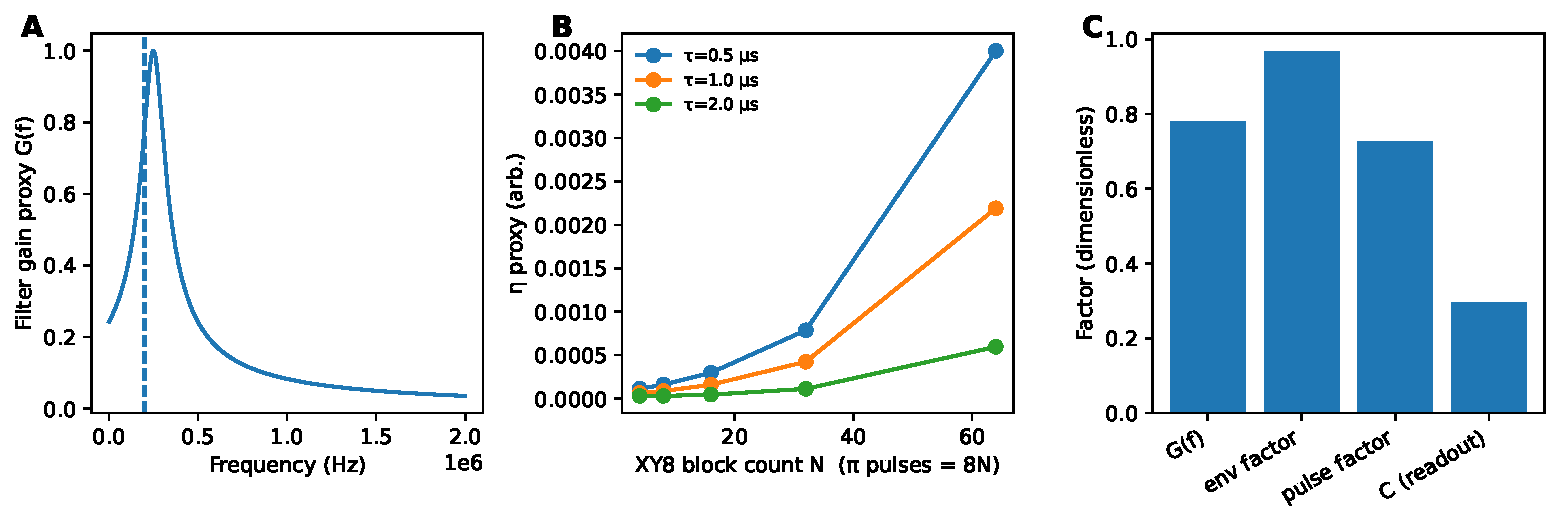
\includegraphics[width=0.90\linewidth]{fig_xy8_qre_nv.pdf}
\caption{\textbf{Quantum resource engineering in NV-center sensing.}
(A) Filter response function $G(f)$ for an XY8 sequence, showing frequency-selective amplification.
(B) Sensitivity proxy as a function of pulse number $N$ and spacing $\tau$, demonstrating a finite optimal regime.
(C) Decomposition of sensing performance into resource factors, including filter gain, environmental coherence, pulse fidelity, and readout contrast.
These results show that optimal sensing arises from a structured balance of competing quantum resources, providing a control-side case study of the EDT finite-regime logic.}
\label{fig:fig5_nvdemo}
\end{figure*}

\subsection{Cross-Platform Interpretation}

Across computation, measurement, and sensing, the same principle emerges: quantum functionality is determined by the structure of the accessible dynamical manifold rather than by the total size of Hilbert space. The plaquette model provides a minimal dynamical realization of this principle, while the NV platform demonstrates its sensing relevance. EDT therefore establishes a programmable resource framework in which control parameters define and navigate structured manifolds of useful dynamics~\cite{Preskill2018,Verstraete2008}.

\section{Discussion}

\subsection{Interpretation}

The results presented here establish EDT as a unifying framework for understanding how quantum resources become physically usable~\cite{Horodecki2009,Streltsov2017}. Across data-driven analysis, minimal dynamical models, and sensing-oriented control optimization, a consistent picture emerges: useful quantum dynamics arise not from maximal entanglement or unrestricted Hilbert-space exploration, but from a finite regime in which structure, interaction, topology, and dynamics are jointly organized~\cite{Amico2008,Eisert2010}.

A central implication is that quantum advantage should be understood as a problem of resource organization rather than resource amplification~\cite{Preskill2018}. In conventional approaches, increasing interaction strength, circuit depth, or entanglement is often assumed to improve performance. However, the results here show that beyond a finite operating window, dynamics become overdriven, leading to degradation of coherence and correlation. This reveals a fundamental trade-off: the same interactions that generate quantum resources also destabilize them when pushed beyond the structured regime~\cite{Altman2015,Swingle2018}.

The data-driven identification of EDT in K$_3$C$_{60}$ demonstrates that this regime arises directly from microscopic electronic structure~\cite{Gunnarsson1997,Capone2009}. The existence of a finite curvature-defined window $\Delta k_{\mathrm{EDT}}$ shows that non-adiabatic coupling naturally organizes quantum resources into localized regions of momentum space~\cite{Mead1979,Yarkony1996}. This provides a physical origin for structured quantum dynamics. The supplementary archived comparison materials show that the same paired-branch residual scan can be exported to materially different datasets, while also making clear that the strength of the finite-window claim depends on branch provenance and robustness information for the specific material under study.

From a dynamical perspective, the minimal plaquette model shows that the EDT regime is characterized by the coexistence of operator spreading and persistent many-body correlations~\cite{Choi2016,KimHuse2013}. This distinguishes EDT from both weakly interacting systems, where dynamics remain local, and strongly driven systems, where coherence is rapidly lost. Instead, EDT occupies an intermediate regime in which interference is stabilized by topology and constrained by symmetry, leading to dynamically organized entanglement~\cite{Swingle2018}.

The scaling and implementation results further demonstrate that this regime is operationally robust. The persistence of the optimal loop strength $\lambda^\star$ and the EDT score under parameter variation and approximate Trotterization indicates that the regime is not fine-tuned~\cite{Lloyd1996,Childs2019}. This establishes EDT as a practical design principle for quantum technologies, guiding the selection of operating conditions in both digital and analog platforms.

The NV-center sensing results provide a sensing-oriented manifestation of the same principle~\cite{Degen2017,Barry2020}. In NV--XY8 protocols, performance is governed by competing resource factors, including filter gain, coherence time, pulse fidelity, and readout contrast. Optimal sensitivity is achieved within a finite control regime in which these factors are balanced, rather than maximized individually. This behavior mirrors the EDT regime identified in the plaquette model, demonstrating that the same structured trade-offs govern both abstract quantum dynamics and experimentally relevant control landscapes~\cite{Casola2018}.

\paragraph*{Relation to superconductivity and electron--phonon theory.}

The curvature-based origin of EDT connects directly to the microscopic theory of superconductivity. In the Bardeen--Pines formulation, electron--phonon interactions renormalize the electronic potential through dynamical screening, producing an effective attractive interaction that underlies BCS pairing~\cite{BardeenPines1955,BCS1957}. These interactions arise from the same dependence of electronic energies on lattice coordinates that generates the non-adiabatic coupling fields considered here.

From the EDT perspective, the key quantity is the second-order response of electronic energies to normal-mode coordinates, which captures curvature induced by lattice dynamics. While in conventional superconductivity this curvature contributes to pairing amplitudes, EDT interprets it more broadly as a generator of structured quantum resource manifolds. Regions of enhanced curvature then define finite domains in parameter space where electronic states are strongly coupled, interference is stabilized, and correlated dynamics are supported~\cite{Giustino2017}.

\paragraph*{Relation to Quantum Advantage Paradigms}

Early demonstrations of quantum advantage, such as random-circuit sampling on programmable superconducting processors~\cite{Arute2019}, emphasized the role of large-scale Hilbert-space exploration in generating classically intractable dynamics. In such systems, advantage arises from highly entangled, strongly scrambled states that are difficult to simulate but lack intrinsic structure or direct operational relevance.

In contrast, EDT identifies a distinct regime of quantum dynamics in which entanglement, interference, and correlation are not maximized globally, but instead organized within finite, geometry-aligned manifolds. Within this regime, operator spreading remains structured and compatible with persistent correlations, enabling both controllability and interpretability. This establishes a complementary paradigm in which useful quantum behavior arises not from the size of Hilbert space explored, but from the structure of the accessible dynamical manifold.

\paragraph*{Relation to Prior Work}

The present framework connects several strands of research across quantum physics and quantum information. The role of non-adiabatic coupling and curvature in shaping electronic structure has been extensively studied in the context of electron--phonon interactions and geometric-phase effects~\cite{Mead1979,Yarkony1996,Giustino2017}. In parallel, quantum-information approaches have explored structured representations of many-body states, including tensor-network methods and symmetry-resolved constructions such as Schur transforms and Clebsch--Gordan decompositions~\cite{Schollwock2011,Bacon2006}. EDT links these directions by identifying a physically grounded regime in which microscopic interactions generate structured manifolds that simultaneously organize entanglement, constrain dynamics, and enable efficient representations.

\subsection{Conclusion and Outlook}

We have introduced EDT as a framework in which quantum resources are organized into finite, geometry-aligned manifolds. By combining data-driven analysis of electronic structure with minimal dynamical models and implementation-level scaling, we have shown that useful quantum dynamics arise within a finite regime defined by the interplay of symmetry, interaction, topology, and dynamics.

This regime is both physically grounded and operationally robust. It emerges from microscopic non-adiabatic coupling~\cite{Mead1979,Yarkony1996}, manifests as structured operator dynamics~\cite{Swingle2018}, and remains stable under realistic circuit approximations~\cite{Lloyd1996,Childs2019}. Across materials, dynamical models, and sensing platforms, a consistent picture emerges: quantum functionality is governed by the structure of the accessible dynamical manifold rather than by the size of Hilbert space~\cite{Amico2008,Eisert2010}.

Looking forward, several directions naturally follow. On the materials side, curvature-based identification of EDT provides a route to screening structured quantum regimes in correlated and strongly coupled systems, provided that branch selection and robustness can be documented with the same care as in the K$_3$C$_{60}$ reference case~\cite{Capone2009}. On the algorithmic side, EDT motivates quantum-computation strategies based on navigating structured dynamical manifolds, rather than maximizing circuit depth or entanglement~\cite{Preskill2018}. On the sensing side, platforms such as NV centers provide a practical route for testing finite-regime control optimization under realistic constraints~\cite{Degen2017}.

\section{Methods}

\paragraph*{Electronic Structure and Curvature Analysis}

The data-driven identification of EDT in K$_3$C$_{60}$ is based on curvature-resolved analysis of electronic band structure near the Fermi level~\cite{Gunnarsson1997,Capone2009}. Microscopically, the relevant curvature originates from second-order variations of band energies with respect to normal-mode coordinates,
\begin{equation}
\kappa_{n\alpha} = \frac{\partial^2 E_n}{\partial Q_\alpha^2},
\end{equation}
which quantify the modulation of electronic energies under lattice distortions and encode non-adiabatic electron--phonon coupling~\cite{Mead1979,Yarkony1996,Giustino2017}. As discussed in the Supplement, these curvature terms arise from second-order mixing between electronic states mediated by NACT, extending beyond the Born--Oppenheimer approximation~\cite{BornOppenheimer1927}.

In practice, the K$_3$C$_{60}$ workflow uses mode-resolved curvature traces
\begin{equation}
\kappa_{n\alpha}(k) = \frac{\partial^2 E_n(k,Q_\alpha)}{\partial Q_\alpha^2},
\end{equation}
evaluated along a high-symmetry momentum path for a selected normal mode. Near degeneracies and avoided crossings, curvature is treated within a multi-band subspace, and paired curvature branches are analyzed using local quadratic fits,
\begin{equation}
\kappa_\pm(k) \approx a_\pm (k-k_0)^2 + b_\pm.
\end{equation}
The EDT window $\Delta k_{\mathrm{EDT}}$ is then defined as the maximal interval over which the residual of this quadratic approximation remains below a specified threshold. The main-text quantitative diagnostic is the K$_3$C$_{60}$ analysis, while the supplementary controls use the same candidate-pair scan on archived comparison datasets from V, Na, LaH$_{10}$, and YBa$_2$Cu$_3$O$_7$ to test portability under a common threshold protocol.

\paragraph*{Minimal Dynamical Model}

The dynamical realization of EDT is studied using a four-qubit plaquette Hamiltonian,
\begin{equation}
H =
J \sum_{\langle i,j\rangle} Z_i Z_j
+
h \sum_i X_i
+
\lambda Z_0 Z_1 Z_2 Z_3,
\end{equation}
where the nearest-neighbor $ZZ$ terms provide local couplings, the transverse-field term drives operator spreading, and the plaquette term introduces loop-induced nonlocal correlations. The Hamiltonian is used as a minimal structural model rather than as a quantitatively fitted K$_3$C$_{60}$ Hamiltonian. Time evolution is computed both exactly and using first-order Trotterized implementations~\cite{Lloyd1996,Trotter1959,Suzuki1990,Childs2019}.

\paragraph*{OTOC and Correlation Diagnostics}

Operator spreading is quantified using the out-of-time-ordered echo
\begin{equation}
F(t) = \langle W^\dagger(t)V^\dagger W(t)V\rangle,
\end{equation}
and the plotted OTOC metric is $1-\mathrm{Re}\,F(t)$~\cite{Larkin1969,Maldacena2016,Swingle2018}. In the script workflow this metric is averaged over several initial-state/operator probes rather than being inferred from a single choice. Long-time correlations are characterized by
\begin{equation}
A_{\mathrm{corr}}^{\mathrm{raw}} = \overline{|\langle Z_i Z_{i+1}(t) \rangle|}_{\mathrm{late},\,i},
\end{equation}
while the entanglement contribution is obtained from the late-time one-qubit entropy. The dynamical EDT score is defined as
\begin{equation}
S_{\mathrm{dyn}}(\lambda) =
A_{\mathrm{spread}}(\lambda)\,
A_{\mathrm{corr}}(\lambda)\,
A_{\mathrm{stability}}(\lambda),
\end{equation}
where $A_{\mathrm{spread}}$ is the normalized mid-time OTOC amplitude, $A_{\mathrm{corr}}$ is the normalized late-time correlation persistence, and $A_{\mathrm{stability}}$ is an intermediate-entropy factor peaked away from both zero and saturation.

\paragraph*{Trotterized Implementation and Scaling}

Time evolution under the Hamiltonian is approximated using first-order Trotterization, with circuit depth and gate count scaling linearly with evolution time~\cite{Trotter1959,Suzuki1990,Lloyd1996,Childs2019}. Observable errors are quantified by comparing exact and Trotterized expectation values~\cite{BerryAhokasCleveSanders2007}. The finite dynamical regime is characterized by sweeping the loop strength $\lambda$ and identifying the optimal value $\lambda^\star$ that maximizes $S_{\mathrm{dyn}}$. Robustness is evaluated by repeating the sweep for several transverse-field values $h$ and several fixed $J$ values, and by comparing exact and Trotterized evolutions.

\paragraph*{NV-Center Sensing Model}

Quantum sensing in NV-center ensembles is analyzed within a quantum resource engineering framework using a rate-based model~\cite{NVRateModel2023,Degen2017,Barry2020}. For XY8 dynamical-decoupling sequences, the control parameter set is
\begin{equation}
\mathcal{C} = \{P_{\mathrm{laser}},\, t_{\mathrm{read}},\, \Omega_{\mathrm{MW}},\, \tau,\, N_{\pi},\, B_0,\, T,\, \mathrm{strain}\},
\end{equation}
and the effective resource vector is
\begin{equation}
\mathcal{R} = \{R_{\mathrm{ph}},\, C,\, T_2(N_{\pi}),\, \chi(\omega),\, \mathrm{duty}\}.
\end{equation}
Here $R_{\mathrm{ph}}$ is the detected photon rate, $C$ is the fluorescence contrast, $T_2(N_{\pi})$ is the coherence time under dynamical decoupling, $\chi(\omega)$ is the filter-function response, and $\mathrm{duty}$ accounts for initialization and readout overhead. The sensing proxy is taken to scale as
\begin{equation}
\eta_{\mathrm{AC}}(\omega) \propto \frac{1}{\chi(\omega)\,C\,\sqrt{R_{\mathrm{ph}}\,T_2(N_{\pi})}} \times f_{\mathrm{duty}},
\end{equation}
and parameter sweeps over $(\tau,N_{\pi})$ are used to identify finite optimal operating points.

\subsection{Availability and Declarations}

\paragraph*{Data availability.}
The data supporting the findings of this study are available from the corresponding author upon reasonable request.

\paragraph*{Code availability.}
The code used in this study is available from the corresponding author upon reasonable request and will be made publicly available upon publication. The active reproducibility bundle includes \texttt{scripts/make\_fig2\_k3c60\_edt.py} for the main K$_3$C$_{60}$ diagnostic, \texttt{scripts/make\_figS4\_material\_controls.py} for the supplementary archived cross-material controls, and \texttt{scripts/fig4\_plaquette\_dynamics.py} for the plaquette dynamics sweep.

\paragraph*{Competing interests.}
The authors declare no competing interests.


\bibliography{references}

\end{document}
